\chapter{Funciones}\label{funciones}

La función es, tal vez, uno de los conceptos más importantes en matemáticas, pues gran parte de los demás conceptos matemáticos se basan en el conocimiento de las funciones y sus propiedades. Aunque existen muchos tipos de funciones —por ejemplo, el área de un círculo que depende de su radio, el costo de un envío que depende de su peso, o la velocidad que depende del tiempo \(t\) transcurrido—, las funciones no siempre dependen de una sola variable. Por ejemplo, el volumen de un cilindro depende tanto de su altura como de su radio. 

En esta sección nos enfocaremos inicialmente en las funciones de una variable real y desarrollaremos con detalle este concepto fundamental.


\section{Propiedades básicas}

\begin{definition}[Función]
Una función \( f \) es una regla de correspondencia que asigna a cada elemento \( x \) de un conjunto denominado \textbf{dominio}, un único valor \( f(x) \) en otro conjunto, llamado \textbf{codominio}. 

El conjunto de todos los valores \( f(x) \) obtenidos se denomina \textbf{rango} o \textbf{imagen} de \( f \). Es común decir que $x$ es la variable independiente y $f(x)$ es la variable dependiente además de usar la notación $y=f(x)$ de manera indistinta.
\end{definition}
\begin{prob} \label{ejdominio}
Calcule el dominio de las siguientes funciones
\begin{enumerate}
\item $f(x)=x^2-8x+5.$
\item $f(x)=\sqrt{1-x^2}.$
\item $f(x)=\sqrt{3+x}+\sqrt[4]{7-x}.$
\item $f(x)=\dfrac{x+5}{x-3}$
\end{enumerate}
\begin{myproof}
\begin{enumerate}
\item La función es un polinomio de grado $2$. Los polinomios están definidos para todo $x \in \mathbb{R}$, sin restricciones. Por tanto, \(
\operatorname{Dom}(f) = \mathbb{R}.
\)

\item La raíz cuadrada requiere $1 - x^2 \geq 0$. Factorizamos:
\[
1 - x^2 = (1 - x)(1 + x) \geq 0.
\]
\begin{table}[H]
\centering
\begin{tabular}{|c|c|c|c|}
\hline
Intervalo & $1+x$ & $1-x$ & $(1-x)(1+x)$ \\
\hline $(-\infty,-1)$ & $-$ & $+$ & $-$ \\
\hline $(-1,1)$ & $+$ & $+$ & $+$ \\
\hline $(1,+\infty)$ & $+$ & $-$ & $-$ \\
\hline
\end{tabular}
\caption{Tabla de signos para el problema \ref{ejdominio} }
\end{table}



\item Analizamos cada radical por separado. Para $\sqrt{3+x}$ se cumple que $3 + x \geq 0 \iff x \geq -3$ y para $\sqrt[4]{7-x}$ se tiene que las raíces de índice par requieren radicando $\geq 0$. Así, $7 - x \geq 0 \iff x \leq 7$. Finalmente la suma está definida cuando ambas lo están, por tanto 
\(\operatorname{Dom}(f) = [-3, 7].\)
\item La función está definida para todo número real excepto donde el denominador sea 0. De esta manera, \(\operatorname{Dom}(f) = \mathbb{R}-\lbrace 3 \rbrace.\)
\end{enumerate}
\end{myproof}
\end{prob}


\begin{rem}[Formas de representar una función]
Existen básicamente cuatro formas de representar una función: verbalmente, describiendo en palabras la relación entre variables; numéricamente, mediante una tabla de valores; visualmente, a través de una gráfica; y algebraicamente, por medio de una fórmula explícita. Aclararemos estas formas en el siguiente ejemplo.
\end{rem}

\begin{example}\label{funcioncosto}
Un contenedor rectangular sin tapa tiene un volumen de \(10\,\text{m}^3\). La longitud de su base es dos veces su ancho. El material para la base cuesta \$10 por metro cuadrado y el material para los lados cuesta \$6 por metro cuadrado. Exprese el costo de los materiales como una función del ancho de la base. Dé una representación verbal, numérica, visual y algebraica.

\begin{myproof}
Primero introducimos las variables geométricas del problema. Sea \(x\) el ancho de la base (en metros), \(2x\) la longitud de la base (en metros) y \(h\) la altura del contenedor (en metros). Como el contenedor no tiene tapa, solo hay base y cuatro lados.

La condición de volumen se escribe como
\[
V = (\text{ancho})\cdot(\text{longitud})\cdot(\text{altura}) = x \cdot 2x \cdot h = 2x^{2}h = 10.
\]
Despejamos la altura en función del ancho:
\[
h = \frac{10}{2x^{2}} = \frac{5}{x^{2}}.
\]

Ahora calculamos el área de cada parte para expresar el costo total. 
El área de la base es
\[
A_{\text{base}} = x \cdot 2x = 2x^{2},
\]
y su costo es
\[
C_{\text{base}} = 10 \cdot A_{\text{base}} = 10 \cdot 2x^{2} = 20x^{2}.
\]

El contenedor tiene cuatro lados rectangulares: dos lados de dimensiones \(x \times h\) y dos de dimensiones \(2x \times h\). El área total de los lados es
\[
A_{\text{lados}} = 2(xh) + 2(2xh) = 2xh + 4xh = 6xh.
\]
Sustituimos \(h = \dfrac{5}{x^{2}}\):
\[
A_{\text{lados}} = 6x \cdot \frac{5}{x^{2}} = \frac{30}{x}.
\]
El costo de los lados es entonces
\[
C_{\text{lados}} = 6 \cdot A_{\text{lados}} = 6 \cdot \frac{30}{x} = \frac{180}{x}.
\]

Sumando ambos aportes obtenemos el costo total como función del ancho \(x\):
\[
C(x) = C_{\text{base}} + C_{\text{lados}} = 20x^{2} + \frac{180}{x}.
\]

Podemos ahora presentar las cuatro representaciones de la función costo:

\textbf{Representación verbal:} A cada valor positivo del ancho \(x\) se le asigna el costo total de construir el contenedor, sumando el costo de la base y el de los cuatro lados, donde la longitud es \(2x\) y la altura se ajusta para que el volumen sea \(10\,\text{m}^3\).

\textbf{Representación algebraica:} La función costo en términos del ancho \(x\) está dada por
\[
C(x) = 20x^{2} + \frac{180}{x}, \quad x > 0.
\]

\textbf{Representación numérica:} Podemos elaborar una tabla de valores, eligiendo algunos anchos \(x\) (en metros) y calculando el costo \(C(x)\) (en dólares). Por ejemplo:
\[
\begin{array}{c|c}
x & C(x) \\
\hline
1   & 20(1)^{2} + \dfrac{180}{1}   = 200 \\
1.5 & 20(1.5)^{2} + \dfrac{180}{1.5} = 20\cdot 2.25 + 120 = 165 \\
2   & 20(2)^{2} + \dfrac{180}{2}   = 80 + 90 = 170 \\
2.5 & 20(2.5)^{2} + \dfrac{180}{2.5} = 20\cdot 6.25 + 72 = 197 \\
\end{array}
\]

\textbf{Representación visual:} La representación gráfica consiste en dibujar la curva de la función
\[
y = C(x) = 20x^{2} + \frac{180}{x}, \quad x > 0,
\]
en el plano \(xy\), donde el eje horizontal representa el ancho \(x\) y el eje vertical representa el costo \(C(x)\). Esta gráfica muestra cómo varía el costo total según el ancho de la base.
\begin{figure}[H]
\centering
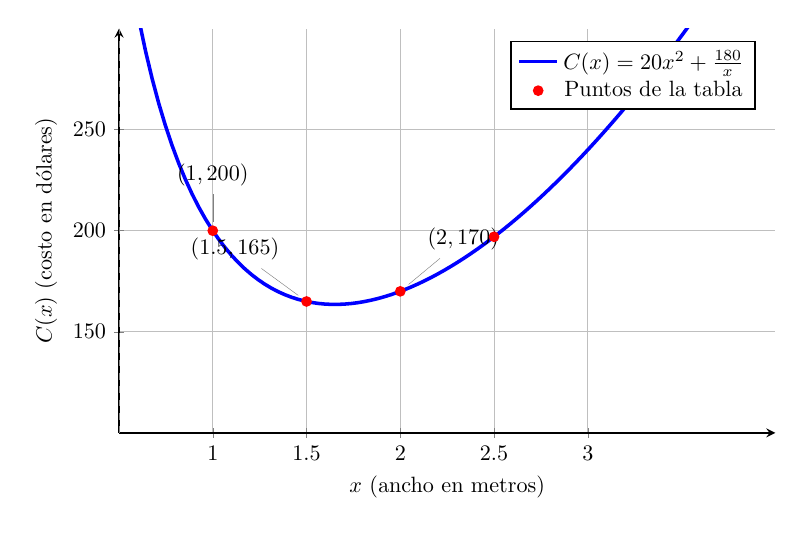
\begin{tikzpicture}[scale=0.8]
% Definir la función
\begin{axis}[
    width=12cm,
    height=8cm,
    xlabel={$x$ (ancho en metros)},
    ylabel={$C(x)$ (costo en dólares)},
    xmin=0.5, xmax=4,
    ymin=100, ymax=300,
    grid=major,
    axis lines=left,
    xtick={1,1.5,2,2.5,3},
    ytick={150,200,250},
    legend pos=north east,
    domain=0.5:4,
    samples=100,
    thick
]

% Graficar la función C(x)
\addplot[blue, ultra thick] {20*x^2 + 180/x};
\addlegendentry{$C(x)=20x^2+\frac{180}{x}$}

% Marcar los puntos de la tabla numérica
\addplot[red, mark=*, only marks] coordinates {
    (1,200)
    (1.5,165)
    (2,170)
    (2.5,197)
};
\addlegendentry{Puntos de la tabla}

% Etiquetas de los puntos clave
\node[pin=90:{$(1,200)$}] at (axis cs:1,200) {};
\node[pin=120:{$(1.5,165)$}] at (axis cs:1.5,165) {};
\node[pin=60:{$(2,170)$}] at (axis cs:2,170) {};

% Línea vertical en x=0 (asíntota)
\draw[dashed, gray] (axis cs:0.5,100) -- (axis cs:0.5,300) node[above right] {asíntota};

\end{axis}
\end{tikzpicture}
\caption{Figura del ejemplo \ref{funcioncosto}}

\end{figure}
Con esto hemos descrito el costo como función del ancho en sus cuatro formas: verbal, numérica, visual y algebraica.
\end{myproof}
\end{example}
Aunque conocer las cuatro representaciones de una función (verbal, numérica, algebraica y gráfica) es fundamental, en ocasiones una resulta más conveniente que las demás según el contexto. Por ello, es esencial seleccionar la representación más adecuada para cada situación particular. La siguiente es una propiedad clave para identificar gráficas de funciones:

\begin{rem}[Prueba de la recta vertical]


Una curva en el plano $XY$ es la gráfica de una función $y=f(x)$ si y solo si ninguna recta vertical se interseca con la curva en más de un punto. 

Por ejemplo, la circunferencia de radio $1$ centrada en el origen, dada por $x^2 + y^2 = 1$, no representa una función de $x$, ya que una recta vertical como $x=0.5$ la interseca dos veces.

\begin{figure}[H]
\centering
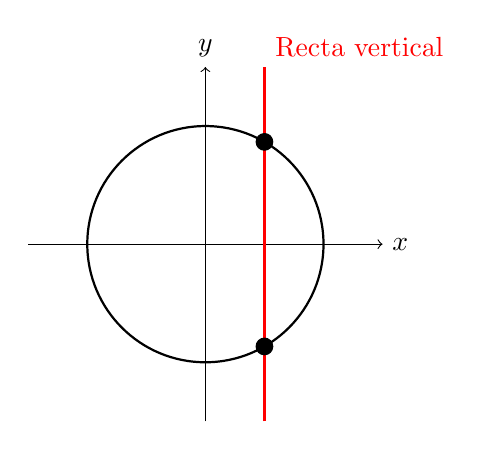
\begin{tikzpicture}[scale=1.5]
\draw[->] (-1.5,0) -- (1.5,0) node[right] {$x$};
\draw[->] (0,-1.5) -- (0,1.5) node[above] {$y$};
\draw[thick] (0,0) circle (1cm);
\draw[red, very thick] (0.5, -1.5) -- (0.5,1.5) node[above right] {Recta vertical};
\filldraw (0.5, 0.866) circle (2pt) node[above right] {};
\filldraw (0.5, -0.866) circle (2pt) node[below right] {};
\end{tikzpicture}
\caption{Circunferencia unitaria fallando la prueba de la recta vertical.}
\label{fig:circulo-vertical}
\end{figure}

\end{rem}

\begin{definition}[Funciones crecientes y decrecientes] Una función $f$ se denomina \textbf{creciente} sobre un intervalo $I$ si $f(x_1)<f(x_2)$ siempre que $x_1<x_2$ para todo $x\in I.$ De manera análoga, $f$ se denomina \textbf{decreciente} sobre un intervalo $I$ si $f(x_1)>f(x_2)$ siempre que $x_1<x_2\in I.$
\end{definition}

\begin{example} 
Determine los intervalos donde la función $f(x)=x^2$ es creciente o decreciente.
\begin{myproof} Hagamos inicialmente un bosquejo de la función

\begin{figure}[H]
\centering
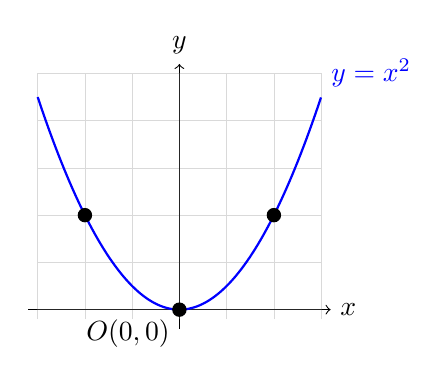
\begin{tikzpicture}[scale=1.2]
% Ejes
\draw[->] (-1.6,0) -- (1.6,0) node[right] {$x$};
\draw[->] (0,-0.2) -- (0,2.6) node[above] {$y$};

% Malla ligera cerca de cero
\draw[help lines, step=0.5cm, opacity=0.3] (-1.5,-0.1) grid (1.5,2.5);

% Bosquejo de y = x^2 cerca de cero
\draw[thick, blue, domain=-1.5:1.5, samples=100] plot (\x, {\x*\x}) 
    node[above right] {$y = x^2$};

% Puntos clave cerca de cero
\filldraw (0,0) circle (2pt) node[below left] {$O(0,0)$};
\filldraw (1,1) circle (2pt) node[above right] {};
\filldraw (-1,1) circle (2pt) node[above left] {};

\end{tikzpicture}
\caption{Bosquejo de $y=x^2.$}
\label{fig:parabola-cero}
\end{figure}


Visualmente se observa que la función tiene forma de parábola y vértice en $x=0$, sugiriendo comportamiento diferente a cada lado. Analizamos por casos.

\textbf{Caso 1: $x \geq 0$ (intervalo $[0, +\infty)$).} Sean $x_1, x_2 \geq 0$ con $x_1 < x_2$. Entonces $x_2 - x_1 > 0$.

Calculamos:
\begin{align*}
f(x_2) - f(x_1) &= x_2^2 - x_1^2 = (x_2 - x_1)(x_2 + x_1).
\end{align*}
Como $x_2 - x_1 > 0$ y $x_2 + x_1 \geq x_1 + x_1 = 2x_1 \geq 0$, se tiene $f(x_2) - f(x_1) > 0 \iff f(x_2) > f(x_1)$.

Por tanto, $f$ es estrictamente creciente en $[0, +\infty)$.


\textbf{Caso 2: $x \leq 0$ (intervalo $(-\infty, 0]$).} Sean $x_1, x_2 \leq 0$ con $x_1 < x_2 \leq 0$. Entonces $x_2 - x_1 > 0$.

Ahora:
\begin{align*}
f(x_2) - f(x_1) &= x_2^2 - x_1^2 = (x_2 - x_1)(x_2 + x_1).
\end{align*}
Como $x_2 - x_1 > 0$ pero $x_2 + x_1 \leq x_2 + x_2 = 2x_2 \leq 0$, se tiene $f(x_2) - f(x_1) < 0 \iff f(x_2) < f(x_1)$.

Por tanto, $f$ es estrictamente decreciente en $(-\infty, 0]$.

\end{myproof}
\end{example}

El ejemplo anterior se resolverá con mayor facilidad más adelante, luego de estudiar la derivada. Mientras tanto, observe que hay algunas formas adicionales de representar funciones:

\begin{example}[Función definida por partes] 
A veces las funciones se describen mediante diferentes fórmulas o expresiones en distintas partes de sus dominios. Trace la gráfica de la siguiente función definida por partes: 
\[
f(x) = 
\begin{cases}
3-\dfrac{1}{2}x & \text{si } x < 2 \\
2x-5 & \text{si } x \geq 2 \\
\end{cases}
\]
\begin{myproof}
El dominio de la función es $\mathbb{R}$. Graficamos cada pieza por separado: Para $x<2$: $y=3 - \frac{1}{2}x$ es recta decreciente con pendiente $-\frac{1}{2}$, círculo \textbf{abierto} en $x=2$ ($y=2$) y para $x \geq 2$: $y=2x-5$ es recta creciente con pendiente $2$, círculo \textbf{lleno} en $x=2$ ($y=-1$).

\begin{figure}[H]
\centering
\begin{tikzpicture}[scale=1.2]
\draw[->] (0, -2) -- (0, 4) node[right] {$y$};
\draw[->] (-0.5, 0) -- (4.5, 0) node[right] {$x$};
\node at (2, -0.3) {$2$};

% Rama 1: x < 2, 3 - 0.5x (círculo abierto en x=2)
\draw[thick, blue, domain=-0.5:1.99, samples=50] plot (\x, {3 - 0.5*\x});
\fill[white, opacity=1] (2,2) circle (3pt); % Círculo abierto
\draw[blue] (2,2) circle (3pt);

% Rama 2: x >= 2, 2x-5 (círculo lleno en x=2)
\draw[thick, red, domain=2:4.5, samples=50] plot (\x, {2*\x - 5});
\filldraw[red] (2,-1) circle (3pt);

\node[blue] at (1,3.2) {$3 - \frac{1}{2}x$ ($x<2$)};
\node[red] at (3.5,2) {$2x-5$ ($x \geq 2$)};
\end{tikzpicture}
\caption{Gráfica de la función $f(x)$ definida por partes.}
\end{figure}
\end{myproof}
\end{example}

\begin{definition}[Funciones pares e impares]
Una función $f: D \to \mathbb{R}$ se clasifica como \textbf{par} si satisface la simetría respecto al eje $y$:
\[
f(-x) = f(x) \quad \forall x \in D \cap (-D),
\]
donde $D \cap (-D) \neq \emptyset$ asegura que el dominio contenga pares simétricos respecto al origen. 

Análogamente, se clasifica como \textbf{impar} si exhibe simetría puntual respecto al origen:
\[
f(-x) = -f(x) \quad \forall x \in D \cap (-D).
\]
\end{definition}


\begin{example}
La función $f(x) = x^2$ es par, ya que:
\[
f(-x) = (-x)^2 = x^2 = f(x) \quad \forall x \in \mathbb{R}.
\]
Asimismo, la función $f(x) = x^3$ es impar, pues:
\[
f(-x) = (-x)^3 = -x^3 = -f(x) \quad \forall x \in \mathbb{R}.
\]
Estas identidades algebraicas verifican las respectivas simetrías geométricas en sus gráficas.
\end{example}

En la sección subsiguiente se presentará un catálogo más completo de funciones elementales, permitiendo explorar sistemáticamente estas propiedades simétricas y otras características relevantes del análisis funcional.



\section{Funciones elementales fundamentales}

Existe un catálogo básico de funciones elementales fundamentales ---conocidas también como \emph{modelos matemáticos esenciales}---, que incluye la función potencia, la exponencial, la logarítmica, las trigonométricas y las trigonométricas inversas. Estas constituyen la base para la construcción de modelos matemáticos más complejos, y en este capítulo se analizarán detalladamente sus dominios, rangos y gráficas.


\begin{definition}[Función potencia]
Sea $r \in \mathbb{Q}$ un número racional escrito en su forma reducida $r = \frac{p}{q}$, donde $p \in \mathbb{Z}$ es un entero y $q \in \mathbb{N}^+$ es un entero positivo con $\gcd(p,q)=1$. La función potencia $f(x) = x^r = \sqrt[q]{x^p}$ tiene dominio que depende de la paridad del denominador $q$ y la señal de $r$:

\begin{itemize}
\item Si $q$ es \textbf{impar}, la raíz $q$-ésima está definida para todo $x \in \mathbb{R}$, por lo que $\operatorname{Dom}(f) = \mathbb{R}$.
\item Si $q$ es \textbf{par}, la raíz $q$-ésima de números negativos no está definida en reales, requiriendo $x^p \geq 0$. Para $p$ impar esto equivale a $x \geq 0$, dando $\operatorname{Dom}(f) = [0, +\infty)$.
\item Si $r < 0$, la expresión involucra división por $x^{-r}$, requiriendo excluir $x=0$: $\operatorname{Dom}(f) = \mathbb{R} \setminus \{0\}$ (o $(0,+\infty)$ si $q$ par).
\end{itemize}

Como casos particulares, para enteros positivos $n \in \mathbb{N}$, $f(x) = x^n$ es un polinomio definido en todo $\mathbb{R}$. Para enteros negativos $n < 0$, $f(x) = x^n = \frac{1}{x^{-n}}$ está definida en $\mathbb{R} \setminus \{0\}$.

Estas reglas garantizan que $x^r$ produzca valores reales para todo $x$ en su dominio respectivo.
\end{definition}





\begin{example}[Ejemplos de funciones potencia elementales] Listamos algunos ejemplos representativos
\begin{figure}[h]
\centering
\begin{tikzpicture}[scale=0.8]
\draw[->] (-2,0) -- (2,0) node[right] {$x$};
\draw[->] (0,-1.5) -- (0,2) node[above] {$y$};
\draw[thick, domain=-1.8:1.8, samples=100] plot (\x, {\x});
\node[above right] at (1.5,1.5) {$f(x)=x$};
\end{tikzpicture}
\caption{$f(x)=x$: $\operatorname{Dom} = \mathbb{R}$.}
\end{figure}


\begin{figure}[H]
\centering
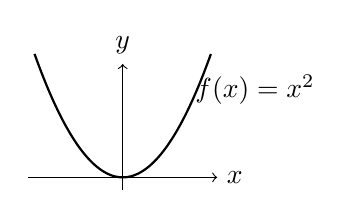
\begin{tikzpicture}[scale=0.8]
\draw[->] (-1.5,0) -- (1.5,0) node[right] {$x$};
\draw[->] (0,-0.2) -- (0,1.8) node[above] {$y$};
\draw[thick, domain=-1.4:1.4, samples=100] plot (\x, {\x*\x});
\node[above right] at (1,1) {$f(x)=x^2$};
\end{tikzpicture}
\caption{Función cuadrática $f(x)=x^2$: $\operatorname{Dom} = \mathbb{R}$.}
\end{figure}

\begin{figure}[H]
\centering
\begin{tikzpicture}[scale=0.8]
\draw[->] (-1.5,0) -- (1.5,0) node[right] {$x$};
\draw[->] (0,-1.2) -- (0,1.8) node[above] {$y$};
\draw[thick, domain=-1.4:1.4, samples=100] plot (\x, {\x*\x*\x});
\node[above right] at (1,1) {$f(x)=x^3$};
\end{tikzpicture}
\caption{Función cúbica $f(x)=x^3$: $\operatorname{Dom} = \mathbb{R}$.}
\end{figure}

\begin{figure}[H]
\centering
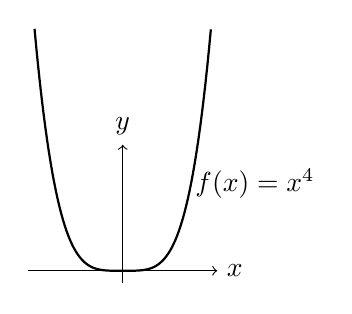
\begin{tikzpicture}[scale=0.8]
\draw[->] (-1.5,0) -- (1.5,0) node[right] {$x$};
\draw[->] (0,-0.2) -- (0,2) node[above] {$y$};
\draw[thick, domain=-1.4:1.4, samples=100] plot (\x, {\x*\x*\x*\x});
\node[above right] at (1,1) {$f(x)=x^4$};
\end{tikzpicture}
\caption{Función $f(x)=x^4$: $\operatorname{Dom} = \mathbb{R}$, par.}
\end{figure}

\begin{figure}[H]
\centering
\begin{tikzpicture}[scale=0.4]
\draw[->] (-2,0) -- (2,0) node[right] {$x$};
\draw[->] (0,-2) -- (0,3) node[above] {$y$};
\draw[thick, blue, domain=-1.8:-0.1, samples=100] plot (\x, {1/\x});
\draw[thick, blue, domain=0.1:1.8, samples=100] plot (\x, {1/\x});
\node[blue, above right] at (1.2,1) {$f(x)=1/x$};
\end{tikzpicture}
\caption{Función recíproca $f(x)=1/x$: $\operatorname{Dom} = \mathbb{R} \setminus \{0\}$}
\end{figure}



\begin{figure}[H]
\centering
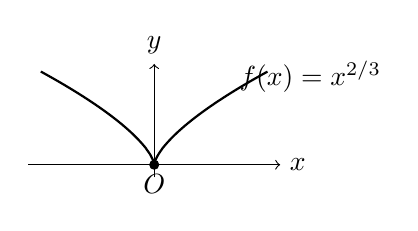
\begin{tikzpicture}[scale=0.8]
\draw[->] (-2,0) -- (2,0) node[right] {$x$};
\draw[->] (0,-0.2) -- (0,1.6) node[above] {$y$};
\draw[thick, domain=-1.8:1.8, samples=200] plot (\x, {abs(\x)^(2/3)});
\filldraw (0,0) circle (2pt) node[below] {$O$};
\node[above right] at (1.2,1) {$f(x)=x^{2/3}$};
\end{tikzpicture}
\caption{Función $x^{2/3}$: $\operatorname{Dom} = \mathbb{R}$.}
\end{figure}

\end{example}


\begin{definition}[Función exponencial] Sea $a$ un número real tal que $a>0$ y $a\neq 1.$ Se define la función exponencial como $f(x)=a^{x}.$ El dominio serán todos los números reales.
\end{definition}

\begin{example}[Ejemplos de funciones exponenciales]
Los siguientes son ejemplos de funciones exponenciales:

 \begin{figure}[H]
\centering
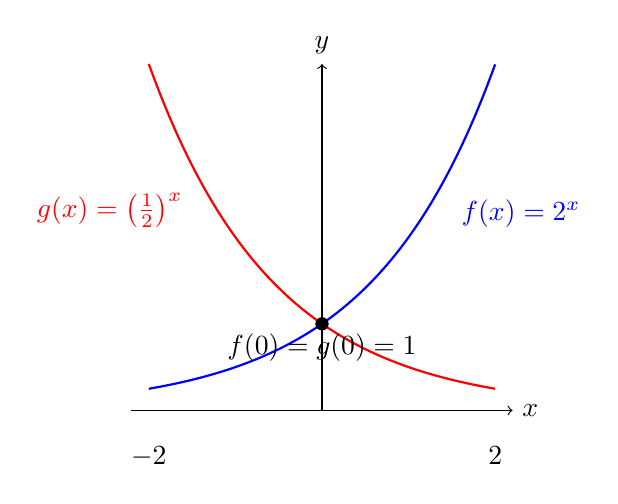
\begin{tikzpicture}[scale=1.1]
% Ejes comunes
\draw[->] (-2.2,0) -- (2.2,0) node[right] {$x$};
\draw[->] (0,0) -- (0,4) node[above] {$y$};

% f(x) = 3^x (creciente, base >1)
\draw[thick, blue, domain=-2:2, samples=100] plot (\x, {2^\x});
\node[blue, above right] at (1.5,2) {$f(x)=2^x$};

% g(x) = (1/2)^x = 2^{-x} (decreciente, 0<base<1)
\draw[thick, red, domain=-2:2, samples=100] plot (\x, {(1/2)^\x});
\node[red, above left] at (-1.5,2) {$g(x)=\left(\frac{1}{2}\right)^x$};

% Puntos clave
\filldraw (0,1) circle (2pt) node[below] {$f(0)=g(0)=1$};
\node at (2,-0.3) [below] {$2$};
\node at (-2,-0.3) [below] {$-2$};
\end{tikzpicture}
\caption{Exponenciales: $f(x)=2^x$ ($\operatorname{Dom}=\mathbb{R}, y>0$), $g(x)=(1/2)^x$ (asíntota $y=0$).}
\label{fig:exp-3-1/5}
\end{figure}
\end{example}

\begin{definition}[Función logarítmica]
Sea $a > 0$, $a \neq 1$ una base válida. La \textbf{función logarítmica} $f(x) = \log_a x$ se define como la función inversa de la exponencial $a^x$, satisfaciendo la propiedad fundamental:
\[
a^{\log_a x} = x = \log_a (a^x) \quad \forall x > 0.
\]
Su dominio natural es $(0, +\infty)$ y su rango es $\mathbb{R}$, siendo estrictamente creciente si $a > 1$ y estrictamente decreciente si $0 < a < 1$.
\end{definition}

\begin{example}[Funciones logarítmicas elementales]
Consideremos dos casos representativos:

\textbf{a)} $f(x) = \log_2 x$ (base $>1$, creciente):

\begin{figure}[H]
\centering
\begin{tikzpicture}[scale=1.1]
\draw[->] (-0.5,0) -- (3.5,0) node[right] {$x$};
\draw[->] (0,-2) -- (0,2.5) node[above] {$y$};
\draw[thick, blue, domain=0.1:3.2, samples=100] plot (\x, {log2(\x)});
\filldraw (1,0) circle (2pt) node[below] {$1$};
\node[blue, above right] at (2,1.2) {$\log_2 x$};
\end{tikzpicture}
\caption{$\log_2 x$: $\operatorname{Dom}=(0,+\infty)$, pasa por $(1,0)$, creciente.}
\end{figure}
\end{example}

Antes de seguir con el siguiente tipo de funciones, es necesaria la siguiente definición 

\begin{definition}[Función periódica]
Una función $f: D \to \mathbb{R}$ se denomina \textbf{periódica} si existe un número real positivo $T > 0$, llamado \textbf{período} de $f$, tal que:
\[
f(x + T) = f(x) \quad \forall x \in D \text{ con } x + T \in D.
\]

El menor número positivo $T$ que satisface esta condición se conoce como \textbf{período fundamental}. Equivalentemente, $f(x + nT) = f(x)$ para todo entero $n \in \mathbb{Z}$ tal que $x + nT \in D$. 
\end{definition}
\begin{rem}
Las funciones periódicas presentan la propiedad geométrica de que su gráfica se compone de copias trasladas del segmento básico correspondiente a un período. Ejemplos clásicos incluyen las funciones trigonométricas, donde $\sin x$ y $\cos x$ tienen período fundamental $2\pi$, mientras que $\tan x$ tiene período $\pi$.
\end{rem}


\begin{definition}[Funciones trigonométricas fundamentales]
Las \textbf{funciones trigonométricas fundamentales} se definen para $x \in \mathbb{R}$ medido en radianes, originadas en las razones trigonométricas de un ángulo en el círculo unitario. Se distinguen seis funciones periódicas con período fundamental $2\pi$ (excepto las secantes y cosecantes), cuyos dominios, rangos y comportamientos se detallan a continuación:

\begin{itemize}
\item $\sin x$: $\operatorname{Dom} = \mathbb{R}$, $\operatorname{Rango} = [-1,1]$, paridad impar.
\item $\cos x$: $\operatorname{Dom} = \mathbb{R}$, $\operatorname{Rango} = [-1,1]$, paridad par.
\item $\tan x$: $\operatorname{Dom} = \mathbb{R} \setminus \left\{\frac{\pi}{2} + k\pi \mid k \in \mathbb{Z}\right\}$, $\operatorname{Rango} = \mathbb{R}$, período $\pi$, paridad impar.
\item $\cot x$: $\operatorname{Dom} = \mathbb{R} \setminus \{k\pi \mid k \in \mathbb{Z}\}$, $\operatorname{Rango} = \mathbb{R}$, período $\pi$, paridad impar.
\item $\sec x = \frac{1}{\cos x}$: $\operatorname{Dom} = \mathbb{R} \setminus \left\{\frac{\pi}{2} + k\pi \mid k \in \mathbb{Z}\right\}$, $\operatorname{Rango} = (-\infty,-1] \cup [1,+\infty)$.
\item $\csc x = \frac{1}{\sin x}$: $\operatorname{Dom} = \mathbb{R} \setminus \{k\pi \mid k \in \mathbb{Z}\}$, $\operatorname{Rango} = (-\infty,-1] \cup [1,+\infty)$.
\end{itemize}
\end{definition}

\begin{example}[Gráficas de las funciones trigonométricas fundamentales] Se presentan a continuación las gráficas de las funciones trigonométricas fundamentales:
\begin{figure}[H]
\centering
% sin x y cos x
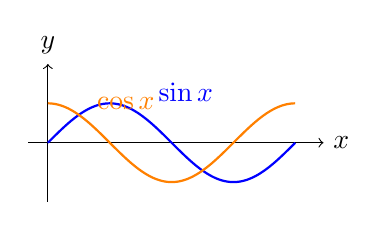
\begin{tikzpicture}[scale=0.5]
\draw[->] (-0.5,0) -- (7,0) node[right] {$x$};
\draw[->] (0,-1.5) -- (0,2) node[above] {$y$};
\draw[thick, blue, domain=0:6.28, samples=150] plot (\x, {sin(\x r)});
\draw[thick, orange, domain=0:6.28, samples=150] plot (\x, {cos(\x r)});
\node[blue, above] at (3.5,0.8) {$\sin x$};
\node[orange, right] at (1,1) {$\cos x$};
\end{tikzpicture}
\caption{$\sin x$, $\cos x$: período $2\pi$, rango $[-1,1]$.}
\end{figure}

\begin{figure}[H]
\centering
% tan x y cot x
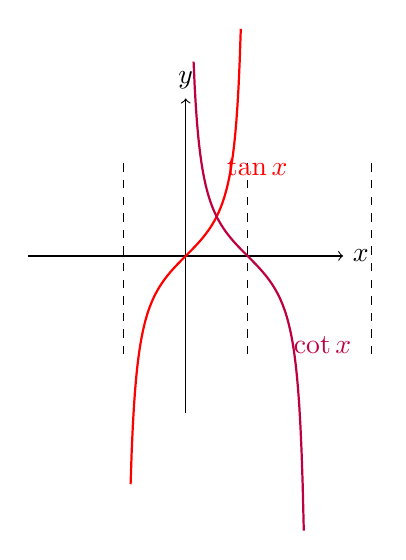
\begin{tikzpicture}[scale=0.5]
\draw[->] (-4,0) -- (4,0) node[right] {$x$};
\draw[->] (0,-4) -- (0,4) node[above] {$y$};
\draw[thick, red, domain=-1.4:1.4, samples=100] plot (\x, {tan(\x r)});
\draw[dashed] (1.57,-2.5) -- (1.57,2.5);
\draw[dashed] (-1.57,-2.5) -- (-1.57,2.5);
\draw[dashed] (4.71,-2.5) -- (4.71,2.5);
\draw[thick, purple, domain=0.2:3, samples=100] plot (\x, {1/tan(\x r)});
\node[red, above right] at (0.8,1.8) {$\tan x$};
\node[purple, below right] at (2.5,-1.8) {$\cot x$};
\end{tikzpicture}
\caption{$\tan x$, $\cot x$: período $\pi$, rango $\mathbb{R}$, asíntotas verticales en $\pi/2.$}
\end{figure}

\begin{figure}[H]
\centering
% sec x y csc x
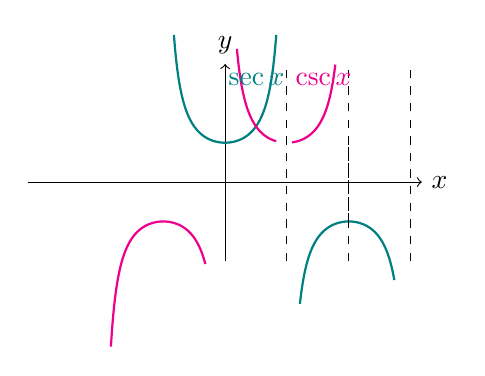
\begin{tikzpicture}[scale=0.5]
\draw[->] (-5,0) -- (5,0) node[right] {$x$};
\draw[->] (0,-2) -- (0,3) node[above] {$y$};
\draw[thick, teal, domain=-1.3:1.3, samples=100] plot (\x, {1/cos(\x r)});
\draw[thick, teal, domain=1.9:4.3, samples=100] plot (\x, {1/cos(\x r)});
\draw[dashed] (1.57,-2) -- (1.57,3);
\draw[dashed] (4.71,-2) -- (4.71,3);
\draw[thick, magenta, domain=0.3:1.3, samples=100] plot (\x, {1/sin(\x r)});
\draw[thick, magenta, domain=1.7:2.8, samples=100] plot (\x, {1/sin(\x r)});
\draw[thick, magenta, domain=-2.9:-0.5, samples=100] plot (\x, {1/sin(\x r)});
\draw[dashed] (3.14,-2) -- (3.14,3);
\draw[dashed] (3.14,-1) -- (3.14,1);
\draw[dashed] (3.14,1) -- (3.14,1);
\node[teal, above] at (0.8,2.2) {$\sec x$};
\node[magenta, above] at (2.5,2.2) {$\csc x$};
\end{tikzpicture}
\caption{$\sec x = 1/\cos x$, $\csc x = 1/\sin x$: rango $\mathbb{R}\setminus(-1,1)$, asíntotas verticales.}
\end{figure}
\end{example}

\begin{definition}[Función compuesta]
Sean $f$ y $g$ dos funciones tales que $g$ está definida en un conjunto $D_g$ y $f$ está definida en un conjunto $D_f$. Si para todo $x \in D_g$ se tiene que $g(x) \in D_f$, se puede definir la \textbf{función compuesta} de $f$ con $g$ como
\[
(f \circ g)(x) = f(g(x)).
\]
El dominio de la función compuesta $f \circ g$ está formado por todos aquellos $x \in D_g$ tales que la imagen $g(x)$ pertenece al dominio de $f$, es decir:
\[
\operatorname{Dom}(f \circ g) = \{\, x \in D_g : g(x) \in D_f \,\}.
\]
\end{definition}

\begin{example}
La función \(
y = \sqrt{1 - x^2}
\) puede interpretarse como una función compuesta de la siguiente manera:
\[
f(u) = \sqrt{u}, \qquad u = g(x) = 1 - x^2.
\]
Aquí, la función interior es $g(x) = 1 - x^2$ y la función exterior es $f(u) = \sqrt{u}$.

El dominio de $g$ es todo $\mathbb{R}$, mientras que el dominio de $f$ es $[0,+\infty)$, pues la raíz cuadrada sólo está definida para argumentos no negativos. Para que la función compuesta $f(g(x)) = \sqrt{1 - x^2}$ esté definida, se requiere que
\[
g(x) = 1 - x^2 \geq 0.
\]
Resolvemos la desigualdad:
\[
1 - x^2 \geq 0 
\iff x^2 \leq 1 
\iff -1 \leq x \leq 1.
\]
Por lo tanto,
\[
\operatorname{Dom}(f \circ g) = [-1,1].
\]
En conclusión, $y = \sqrt{1 - x^2}$ es una función compuesta de $f(u)=\sqrt{u}$ y $g(x)=1-x^2$, cuyo dominio está dado por el intervalo cerrado $[-1,1]$.
\end{example}
\begin{rem}[Composiciones múltiples]
Es posible componer una función múltiples veces formando cadenas de funciones. Por ejemplo, la función
\[
f(x) = \ln(\sin(x^2 + 1))
\]
puede descomponerse en la composición sucesiva de tres funciones elementales:
\[
f(x) = \ln \circ \sin \circ p(x),
\]
donde:
\begin{itemize}
\item $p(x) = x^2 + 1$ (función potencia desplazada),
\item $u = \sin(v)$ con $v = p(x)$, 
\item $y = \ln(u)$ con $u = \sin(p(x))$.
\end{itemize}

Para determinar su dominio, se analizan las restricciones de cada función desde la exterior hacia la interior:
\begin{enumerate}
\item $\ln(u)$ requiere $u > 0$,
\item $\sin(v) \in [-1,1]$, pero debe satisfacer $\sin(v) > 0$,
\item $v = x^2 + 1 \geq 1 > 0$ (siempre definido).
\end{enumerate}
Así, $\operatorname{Dom}(f) = \{x \in \mathbb{R} : \sin(x^2 + 1) > 0\}$, equivalente a los intervalos donde el seno es positivo.
\end{rem}


\begin{definition}[Función elemental]
Una función $f: D \to \mathbb{R}$ se denomina \textbf{elemental} si puede obtenerse a partir de funciones elementales básicas (potencias, exponenciales, logarítmicas, trigonométricas y sus inversas) y constantes reales, mediante un número \emph{finito} de las siguientes operaciones:
\begin{itemize}
\item Suma, resta, multiplicación y división entre funciones,
\item Composición de funciones.
\end{itemize}

Formalmente, el conjunto de funciones elementales $\mathcal{E}$ se define recursivamente como el menor conjunto que contiene:
\begin{itemize}
\item Las funciones potencia $x \mapsto x^r$ ($r \in \mathbb{Q}$),
\item Las exponenciales $x \mapsto a^x$ ($a > 0$, $a \neq 1$),
\item Las logarítmicas $x \mapsto \log_a x$ ($a > 0$, $a \neq 1$), 
\item Las funciones trigonométricas $\sin x$, $\cos x$, $\tan x$, etc.,
\item Las constantes $x \mapsto c$ ($c \in \mathbb{R}$),
\item Y está cerrado bajo suma, producto, cociente y composición.
\end{itemize}

Las expresiones analíticas usuales en cálculo (polinomios, racionales, exponenciales-trigonométricas, etc.) son funciones elementales.
\end{definition}

Un tipo particular de funciones elementales son las \textbf{funciones algebraicas}, que se obtienen únicamente mediante operaciones algebraicas (suma, resta, multiplicación, división y raíces) sobre la variable independiente $x$. Se definen detalladamente a continuación:

\begin{definition}[Función algebraica]
Una función $f: D \to \mathbb{R}$ es \textbf{algebraica} si puede expresarse mediante una expresión finita que involucre únicamente la variable $x$, números reales y las operaciones de suma, resta, multiplicación, división y extracción de raíces $n$-ésimas (con $n \in \mathbb{N}^+$). Equivalentemente, satisface una ecuación polinómica con coeficientes reales:
\[
P(x, f(x)) = 0,
\]
donde $P$ es un polinomio en dos variables.
\end{definition}

\begin{definition}[Función lineal]
Una función $f: \mathbb{R} \to \mathbb{R}$ es \textbf{lineal} si tiene la forma
\[
f(x) = mx + b,
\]
donde $m, b \in \mathbb{R}$ son constantes. Aquí $m$ es la \textbf{pendiente} y $b$ el \textbf{intercepto} con el eje $y$. Su dominio y rango son $\mathbb{R}$, y es inyectiva si $m \neq 0$.
\end{definition}

\begin{definition}[Función polinómica]
Una función $f: \mathbb{R} \to \mathbb{R}$ es \textbf{polinómica} si se expresa como
\[
f(x) = a_n x^n + a_{n-1} x^{n-1} + \cdots + a_1 x + a_0,
\]
donde $n \in \mathbb{N} \cup \{0\}$ es el \textbf{grado}, $a_i \in \mathbb{R}$ y $a_n \neq 0$. Su dominio es $\mathbb{R}$. Cuando $n \geq 2$, se clasifican según su grado (cuadrática $n=2$, cúbica $n=3$, etc.).
\end{definition}

\begin{definition}[Función racional]
Una función $f: D \to \mathbb{R}$ es \textbf{racional} si es un cociente de dos polinomios:
\[
f(x) = \frac{P(x)}{Q(x)},
\]
donde $P, Q$ son polinomios con $Q \not\equiv 0$. Su dominio es
\[
D = \mathbb{R} \setminus \{x \in \mathbb{R} : Q(x) = 0\}.
\]
Las asíntotas y discontinuidades se determinan por los ceros del denominador.
\end{definition}

\begin{definition}[Función irracional]
Una función $f: D \to \mathbb{R}$ es \textbf{irracional} (o radical) si en su expresión analítica aparece al menos una raíz $n$-ésima con $n \geq 2$. El dominio se restringe por las condiciones de definición de las raíces:
\[
\sqrt[n]{P(x)} \quad \text{requiere } P(x) \geq 0 \text{ si } n \text{ par}.
\]
Ejemplos: $f(x) = \sqrt{x}$, $g(x) = \sqrt[3]{x^2 + 1}$.
\end{definition}

Las funciones que no son algebraicas se denominan \textbf{trascendentes}. Ejemplos incluyen las funciones trigonométricas ($y = \cos x$), exponenciales ($y = 10^x$) y logarítmicas ($y = \ln x$), cuya definición trasciende las operaciones algebraicas elementales.


\section{Transformaciones de funciones}

A partir de las funciones básicas estudiadas previamente, las combinaciones de funciones se producen de manera natural: $(f+g)(x)=f(x)+g(x),$ $(f-g)(x)=f(x)-g(x),$ $(fg)(x)=f(x)g(x),$ y $(\dfrac{f}{g})(x)=\dfrac{f(x)}{g(x)}$ con $g(x)\neq 0.$  Ahora, es posible generar nuevas funciones mediante \textbf{transformaciones geométricas} de sus gráficas: traslaciones, dilataciones, compresiones y reflexiones. Estas operaciones preservan las propiedades fundamentales de la función original, modificando únicamente su posición y escala. 

Dados $h, k \in \mathbb{R}$ y $y = f(x)$, las siguientes transformaciones desplazan la gráfica de $f$:

\begin{itemize}
\item $y = f(x - h)$: \textbf{Traslación horizontal} de $h$ unidades ($h > 0$ hacia la derecha, $h < 0$ hacia la izquierda).
\item $y = f(x) + k$: \textbf{Traslación vertical} de $k$ unidades ($k > 0$ hacia arriba, $k < 0$ hacia abajo).
\item $y = f(x - h) + k$: \textbf{Traslación combinada} (horizontal $h$, vertical $k$).
\end{itemize}

\begin{figure}[H]
\centering
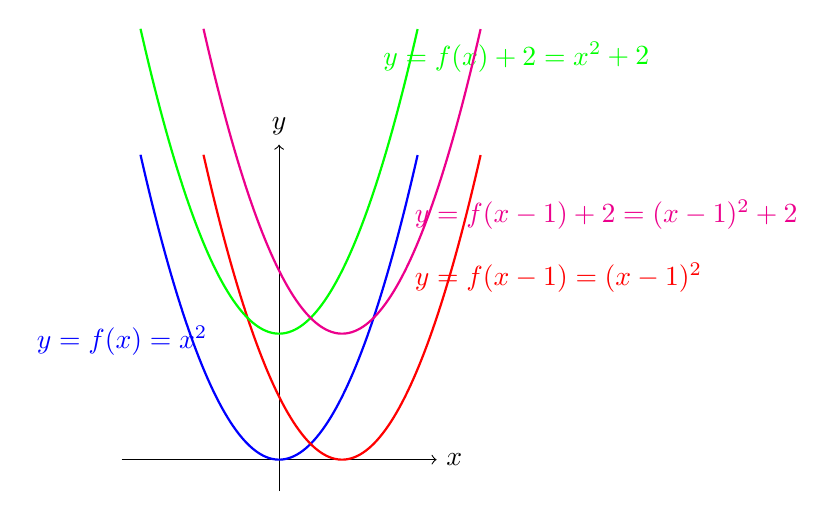
\begin{tikzpicture}[scale=0.8]
% Original: y = (x)^2 = x^2

\draw[->] (-2.5,0) -- (2.5,0) node[right] {$x$};
\draw[->] (0,-0.5) -- (0,5) node[above] {$y$};
\draw[blue,thick, domain=-2.2:2.2, samples=100] plot (\x, {\x*\x});
\node[blue, above right] at (-4,1.5) {$y = f(x) = x^2$};


% f(x-h) = (x-1)^2, h=1

\draw[red,thick, domain=-1.2:3.2, samples=100] plot (\x, {(\x-1)^2});
\node[red, above right] at (2,2.5) {$y = f(x-1) = (x-1)^2$};


% f(x)+k = x^2 + 2, k=2


\draw[green,thick, domain=-2.2:2.2, samples=100] plot (\x, {\x*\x + 2});
\node[green, above right] at (1.5,6) {$y = f(x)+2 = x^2+2$};


% f(x-h)+k = (x-1)^2 + 2

\draw[magenta,thick, domain=-1.2:3.2, samples=100] plot (\x, {(\x-1)^2 + 2});
\node[magenta, above right] at (2,3.5) {$y = f(x-1)+2 = (x-1)^2+2$};

\end{tikzpicture}
\caption{Traslaciones de $y=x^2$: vértice se desplaza de $(0,0)$ a $(h,k)=(1,2)$.}
\label{fig:traslaciones-parabola}
\end{figure}


Suponga que $c > 0$, $c \neq 1$. Las siguientes transformaciones modifican la escala y orientación:

\begin{itemize}
\item $y = c \cdot f(x)$ ($c > 1$): \textbf{Dilatación vertical} por factor $c$.
\item $y = \frac{1}{c} \cdot f(x)$ ($c > 1$): \textbf{Compresión vertical} por factor $c$.
\item $y = f(c \cdot x)$ ($c > 1$): \textbf{Compresión horizontal} por factor $c$.
\item $y = f\left(\frac{x}{c}\right)$ ($c > 1$): \textbf{Dilatación horizontal} por factor $c$.
\item $y = -f(x)$: \textbf{Reflexión respecto al eje $x$}.
\item $y = f(-x)$: \textbf{Reflexión respecto al eje $y$} (preserva paridad).
\end{itemize}

\begin{figure}[H]
\centering
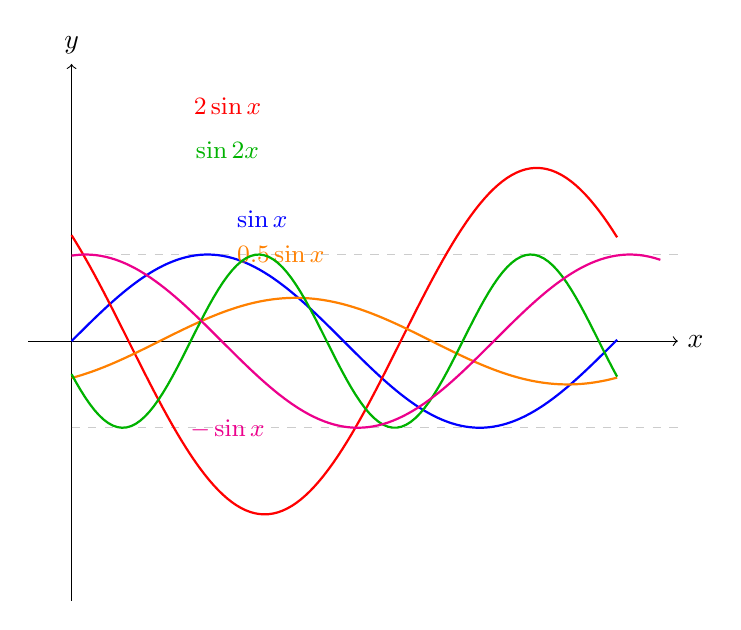
\begin{tikzpicture}[scale=1.1]

% Ejes compartidos
\draw[->] (-0.5,0) -- (7,0) node[right] {$x$};
\draw[->] (0,-3) -- (0,3.2) node[above] {$y$};

% Líneas referencia y=±1
\draw[gray!40,dashed] (0,1) -- (7,1);
\draw[gray!40,dashed] (0,-1) -- (7,-1);

% 1. Original: sin(x)
\draw[thick, blue, domain=0:6.3, samples=120] plot (\x, {sin((\x) r)});
\node[blue, font=\small, above right] at (1.8,1.2) {$\sin x$};

% 2. Amplitud 2: 2sin(x)
\draw[thick, red, domain=0:6.3, samples=120] plot (\x, {2*sin((\x-3.8) r)});
\node[red, font=\small, above] at (1.8,2.5) {$2\sin x$};

% 3. Compresión vertical: 0.5sin(x)
\draw[thick, orange, domain=0:6.3, samples=120] plot (\x, {0.5*sin((\x-7.3) r)});
\node[orange, font=\small, above right] at (1.8,0.8) {$0.5\sin x$};

% 4. Compresión horizontal: sin(2x)
\draw[thick, green!70!black, domain=0:6.3, samples=120] plot (\x, {sin(2*(\x-10.8) r)});
\node[green!70!black, font=\small, above] at (1.8,2) {$\sin 2x$};

% 5. Reflexión vertical: -sin(x)
\draw[thick, magenta, domain=0:6.8, samples=120] plot (\x, {-sin((\x-14.3) r)});
\node[magenta, font=\small, below] at (1.8,-0.8) {$-\sin x$};
\end{tikzpicture}
\caption{Transformaciones superpuestas de $y=\sin x$: amplitud, compresiones y reflexión.}
\label{fig:transformaciones-seno}
\end{figure}



Estas transformaciones permiten sistematizar el análisis gráfico de funciones complejas a partir de funciones básicas conocidas. Para las funciones trigonométricas periódicas $\sin x$ y $\cos x$, cuya forma canónica tiene amplitud $1$, línea media $y=0$ y período $2\pi$, la forma generalizada es $y = C + A \sin \bigl[ a(t + b) \bigr]$ o $y = C + A \cos \bigl[ a(t + b) \bigr],$ donde los parámetros tienen interpretación geométrica precisa:

\begin{itemize}
\item \textbf{Amplitud} $|A|$: distancia máxima desde la línea central hasta los valores extremos.
\item \textbf{Período fundamental} $T = \dfrac{2\pi}{|a|}$: longitud del ciclo completo ($a > 0$ implica compresión, $0 < a < 1$ dilatación horizontal).
\item \textbf{Línea central (desfase vertical)} $C$: valor medio alrededor del cual oscila la función.
\item \textbf{Desfase horizontal} $-b$: desplazamiento lateral del ciclo básico ($\phi = -b$ comúnmente denotado).
\end{itemize}

\begin{figure}[H]
\centering
\begin{tikzpicture}[scale=1.1]
% Ejes
\draw[->] (-0.3,0) -- (7.5,0) node[right] {$t$};
\draw[->] (0,-2.8) -- (0,3) node[above] {$y$};

% Función: y = 0.5 + 1.5 sin(1.2(t + 0.3))
\draw[thick,blue,domain=0:6.5,samples=200,smooth] plot (\x, {0.5 + 1.5*sin(1.2*(\x + 0.3) r)});

% Línea central C=0.5
\draw[dashed,gray,thick] (0,0.5) -- (6.5,0.5) node[right,font=\small] {$y=C=0.5$};

% Amplitud A=1.5
\draw[<->,red,thick] (5.8,0.5) -- (5.8,2) node[midway,right,font=\small] {$|A|=1.5$};

% Período T=2π/1.2 ≈ 5.24
\draw[<->,purple,thick] (0.5,-2.5) -- (5.74,-2.5) node[midway,below,font=\small] {$T=\frac{2\pi}{|1.2|}\approx5.24$};

% Máximos/mínimos para referencia
\filldraw (2.1,2) circle (1.5pt) node[above,font=\tiny] {máx};
\filldraw (4.8,-1) circle (1.5pt) node[below,font=\tiny] {mín};

% Etiqueta función
\node[below=0.1cm,font=\footnotesize] at (3.5,-3.5) {$y = 0.5 + 1.5\sin[1.2(t+0.3)]$};

\end{tikzpicture}
\caption{Componentes de la forma amplitud-fase.}
\label{fig:forma-amplitud-fase}
\end{figure}

Esta parametrización es fundamental para modelar fenómenos oscilatorios (resortes, ondas, circuitos AC) donde la amplitud, frecuencia y fase determinan el comportamiento físico observado.

\section{Funciones inversas}

Muchos fenómenos físicos y matemáticos admiten dos perspectivas complementarias. Considere, por ejemplo, el proceso productivo de una planta de muebles: dada una cantidad de tiempo $t$, podemos determinar la cantidad de muebles producidos $f(t)$; alternativamente, dada una cantidad específica de muebles $y$, podríamos determinar el tiempo necesario para producirlos $t = f^{-1}(y)$. 

En este contexto, si $y = f(t)$ describe la producción acumulada en función del tiempo, la función inversa $f^{-1}$ responde a la pregunta ``¿en cuánto tiempo se producen $y$ muebles?''. Para que esta operación inversa sea bien definida matemáticamente, es necesario garantizar que cada valor $y$ en el rango de $f$ corresponda a un único $x$ en el dominio, condición que formalizamos mediante el concepto de inyectividad.

\begin{definition}[Función inyectiva]
Una función $f: D \to \mathbb{R}$ es \textbf{inyectiva} si para todo par de elementos distintos $x_1, x_2 \in D$ se cumple:
\[
x_1 \neq x_2 \implies f(x_1) \neq f(x_2).
\]
Equivalentemente, $f(a) = f(b)$ implica $a = b$ para todo $a, b \in D$.
\end{definition}

\begin{rem}[Prueba de la recta horizontal]
Una función $f$ es inyectiva si y solo si ninguna recta horizontal $y = k$ (con $k \in \mathbb{R}$) interseca su gráfica en más de un punto. Esta condición geométrica es equivalente a la definición algebraica anterior y proporciona un criterio visual directo para verificar la inyectividad.
\end{rem}

La inyectividad garantiza que cada valor en el rango de $f$ proviene de exactamente un elemento del dominio, condición necesaria y suficiente para que exista una función inversa bien definida $f^{-1}: \operatorname{Ran}(f) \to D$ tal que:
\(
f(f^{-1}(y)) = y \quad \text{y} \quad f^{-1}(f(x)) = x.
\)

Este contexto nos permite introducir rigurosamente el concepto de función inversa.

\begin{definition}[Función inversa]
Sea $f: D \to R$ una función inyectiva, con dominio $D$ y rango (imagen) $R = f(D)$. La \textbf{función inversa} de $f$, denotada por $f^{-1}: R \to D$, se define mediante la relación
\[
f^{-1}(y) = x \;\Longleftrightarrow\; f(x) = y,
\]
para todo $y \in R$ y el único $x \in D$ que satisface dicha igualdad. En otras palabras, $f^{-1}$ “deshace” la acción de $f$.
\end{definition}

\begin{rem}
En general, $f^{-1} \neq \dfrac{1}{f}$: la notación $f^{-1}$ no denota recíproco, sino \emph{función inversa}. Además, cuando $f$ es inyectiva se satisfacen las identidades de composición
\[
f^{-1}(f(x)) = x \quad \text{para todo } x \in D,
\]
\[
f(f^{-1}(y)) = y \quad \text{para todo } y \in R.
\]
Estas igualdades permiten calcular analíticamente la función inversa: dada la ecuación $y = f(x)$, se despeja $x$ en términos de $y$ y, finalmente, se intercambian los roles de las variables ($y$ se renombra como $x$).
\end{rem}

\begin{example}
Determine una fórmula para la inversa de las funciones
\(
y = \frac{4x - 1}{2x + 3} \) y \( y = 2x - 3.\)

\begin{myproof}
\textbf{1. Inversa de } $\displaystyle y = \frac{4x - 1}{2x + 3}$.

Partimos de la ecuación
\[
y = \frac{4x - 1}{2x + 3}.
\]
Paso 1: Intercambiamos $x$ e $y$ para reflejar la inversión:
\[
x = \frac{4y - 1}{2y + 3}.
\]
Paso 2: Despejamos $y$ en términos de $x$. Multiplicamos ambos lados por $2y + 3$:
\[
x(2y + 3) = 4y - 1.
\]
Distribuimos:
\[
2xy + 3x = 4y - 1.
\]
Paso 3: Reagrupamos los términos que contienen $y$ en un lado:
\[
2xy - 4y = -1 - 3x.
\]
Factorizamos $y$:
\[
y(2x - 4) = -1 - 3x.
\]
Paso 4: Despejamos $y$:
\[
y = \frac{-1 - 3x}{2x - 4}.
\]
Podemos multiplicar numerador y denominador por $-1$ para simplificar:
\[
y = \frac{3x + 1}{4 - 2x}.
\]
Por lo tanto,
\[
f^{-1}(x) = \frac{3x + 1}{4 - 2x}.
\]

\textbf{2. Inversa de } $\displaystyle y = 2x - 3$.

Partimos de
\[
y = 2x - 3.
\]
Paso 1: Intercambiamos $x$ e $y$:
\[
x = 2y - 3.
\]
Paso 2: Despejamos $y$ en términos de $x$:
\[
x + 3 = 2y \quad \Longrightarrow \quad y = \frac{x + 3}{2}.
\]
Por tanto,
\[
f^{-1}(x) = \frac{x + 3}{2}.
\]

En ambos casos, puede verificarse la corrección comprobando que $f^{-1}(f(x)) = x$ y $f(f^{-1}(x)) = x$ en los dominios correspondientes.
\end{myproof}
\end{example}

Después del contexto establecido sobre funciones inversas, las funciones trigonométricas básicas ($\sin x$, $\cos x$, etc.) no son globalmente inyectivas debido a su periodicidad. Para definir sus inversas, se restringen a intervalos \emph{principales} donde cada una es biyectiva (inyectiva y sobreyectiva) sobre su rango. Estas funciones trigonométricas inversas se definen a continuación:

\begin{definition}[Funciones trigonométricas inversas]
Las seis funciones trigonométricas inversas fundamentales se definen con dominios y rangos específicos que garantizan su inyectividad:

\begin{center}
\begin{tabular}{|c|l|l|}
\hline
\textbf{Función} & \textbf{Dominio (principal)} & \textbf{Rango} \\
\hline
$\operatorname{arcsin} x$ & $[-1, 1]$ & $\left[-\frac{\pi}{2}, \frac{\pi}{2}\right]$ \\
\hline
$\operatorname{arccos} x$ & $[-1, 1]$ & $[0, \pi]$ \\
\hline
$\operatorname{arctan} x$ & $\mathbb{R}$ & $\left(-\frac{\pi}{2}, \frac{\pi}{2}\right)$ \\
\hline
$\operatorname{arccot} x$ & $\mathbb{R}$ & $(0, \pi)$ \\
\hline
$\operatorname{arcsec} x$ & $(-\infty, -1] \cup [1, +\infty)$ & $[0, \pi] \setminus \{\frac{\pi}{2}\}$ \\
\hline
$\operatorname{arccsc} x$ & $(-\infty, -1] \cup [1, +\infty)$ & $\left[-\frac{\pi}{2}, \frac{\pi}{2}\right] \setminus \{0\}$ \\
\hline
\end{tabular}
\end{center}

\end{definition}

\begin{figure}[H]
\centering
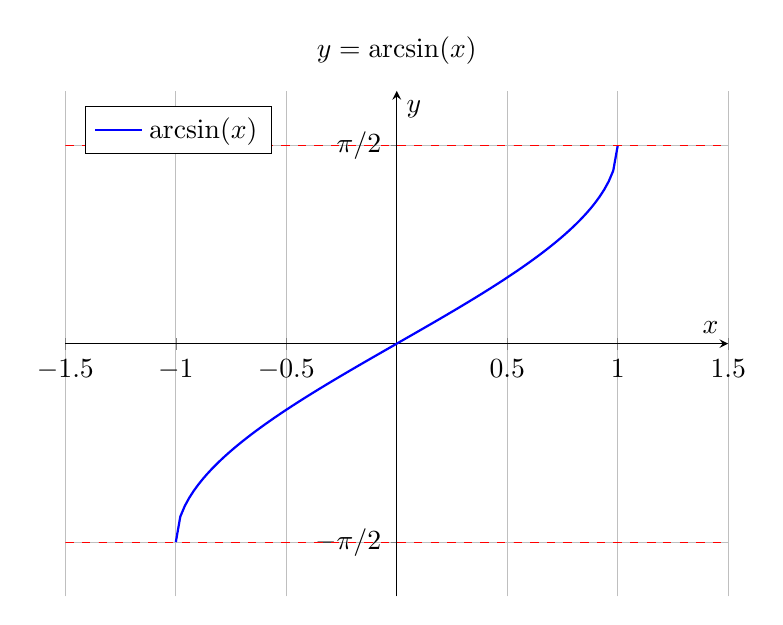
\begin{tikzpicture}
\begin{axis}[
    axis lines = center,
    xlabel = {$x$},
    ylabel = {$y$},
    title = {$y = \arcsin(x)$},
    domain = -1:1,
    samples = 100,
    ymin = -2,
    ymax = 2,
    xmin = -1.5,
    xmax = 1.5,
    grid = major,
    legend pos = north west,
    width = 10cm,
    height = 8cm,
    ytick = {-1.5708, 0, 1.5708},
    yticklabels = {$-\pi/2$, $0$, $\pi/2$},
    trig format plots=rad
]
\addplot[blue, thick] {asin(x)};
\addlegendentry{$\arcsin(x)$}
\addplot[red, dashed, domain=-1.5:1.5] {pi/2};
\addplot[red, dashed, domain=-1.5:1.5] {-pi/2};
\end{axis}
\end{tikzpicture}
\caption{Función arcoseno: dominio $[-1,1]$, rango $[-\pi/2, \pi/2]$}
\end{figure}

\begin{figure}[H]
\centering
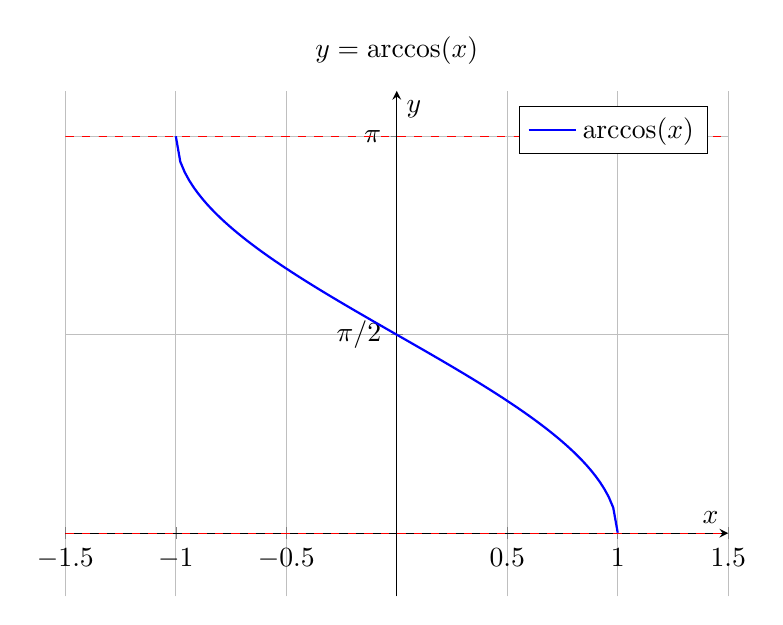
\begin{tikzpicture}
\begin{axis}[
    axis lines = center,
    xlabel = {$x$},
    ylabel = {$y$},
    title = {$y = \arccos(x)$},
    domain = -1:1,
    samples = 100,
    ymin = -0.5,
    ymax = 3.5,
    xmin = -1.5,
    xmax = 1.5,
    grid = major,
    legend pos = north east,
    width = 10cm,
    height = 8cm,
    ytick = {0, 1.5708, 3.14159},
    yticklabels = {$0$, $\pi/2$, $\pi$},
    trig format plots=rad
]
\addplot[blue, thick] {acos(x)};
\addlegendentry{$\arccos(x)$}
\addplot[red, dashed, domain=-1.5:1.5] {pi};
\addplot[red, dashed, domain=-1.5:1.5] {0};
\end{axis}
\end{tikzpicture}
\caption{Función arcocoseno: dominio $[-1,1]$, rango $[0, \pi]$}
\end{figure}

\begin{figure}[H]
\centering
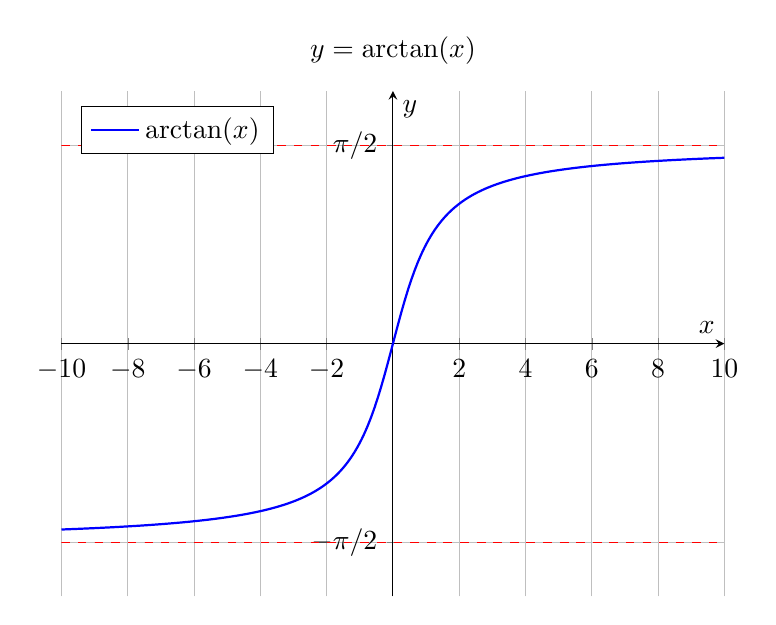
\begin{tikzpicture}
\begin{axis}[
    axis lines = center,
    xlabel = {$x$},
    ylabel = {$y$},
    title = {$y = \arctan(x)$},
    domain = -10:10,
    samples = 200,
    ymin = -2,
    ymax = 2,
    xmin = -10,
    xmax = 10,
    grid = major,
    legend pos = north west,
    width = 10cm,
    height = 8cm,
    ytick = {-1.5708, 0, 1.5708},
    yticklabels = {$-\pi/2$, $0$, $\pi/2$},
    trig format plots=rad
]
\addplot[blue, thick] {atan(x)};
\addlegendentry{$\arctan(x)$}
\addplot[red, dashed, domain=-10:10] {pi/2};
\addplot[red, dashed, domain=-10:10] {-pi/2};
\end{axis}
\end{tikzpicture}
\caption{Función arcotangente: dominio $(-\infty, \infty)$, rango $(-\pi/2, \pi/2)$}
\end{figure}



\section{Operaciones con logaritmos y exponenciales naturales}

Concluimos este capítulo presentando las propiedades fundamentales de las funciones exponenciales y logarítmicas, esenciales para el desarrollo del cálculo diferencial. En particular, se destaca el número \( e \approx 2.71828 \), cuya función asociada \( y = e^x \) tiene pendiente igual a \(1\) en el punto \((0,1)\). Esta característica se demostrará formalmente en el capítulo de límites. Por ahora, estudiaremos las leyes algebraicas que gobiernan las operaciones con potencias, exponentes y logaritmos.

\begin{theorem}[Leyes de los exponentes]
Sean \( a, b > 0 \) y \( x, y \in \mathbb{R} \). Se cumplen las siguientes propiedades:
\begin{enumerate}
    \item \( b^{x+y} = b^x \, b^y \)
    \item \( b^{x-y} = \dfrac{b^x}{b^y} \)
    \item \( (b^x)^y = b^{xy} \)
    \item \( (ab)^x = a^x \, b^x \)
\end{enumerate}
\end{theorem}

\begin{theorem}[Leyes de los logaritmos]
Sea \( b > 0 \) con \( b \neq 1 \), y sean \( x, y > 0 \) y \( r \in \mathbb{R} \). Entonces se verifican las siguientes propiedades:
\begin{enumerate}
    \item \( \log_b(xy) = \log_b x + \log_b y \)
    \item \( \log_b\!\left(\dfrac{x}{y}\right) = \log_b x - \log_b y \)
    \item \( \log_b(x^r) = r\,\log_b x \)
\end{enumerate}
Además, la definición de logaritmo establece la equivalencia \(
\log_b x = y \quad \Longleftrightarrow \quad b^y = x.
\)
\end{theorem}

\begin{definition}[Función logaritmo natural]
El logaritmo natural \(\ln x\) es el logaritmo de base \(e\), es decir \(
\ln x = \log_e x.
\)
Para todo \( x > 0 \) y \( y \in \mathbb{R} \) se cumple 
\(
\ln x = y \iff e^y = x,$ $\ln(e^x) = x, $ y $e^{\ln x} = x.$ En particular, en \(x = 1\), se obtiene \(
\ln e = 1.
\)
\end{definition}

\begin{theorem}[Cambio de base a logaritmos naturales]
Sea \( b > 0 \) y \( b \neq 1 \). Se cumple que \(
\log_b x = \frac{\ln x}{\ln b}.
\)
\end{theorem}

\begin{proof}
Sea \( y = \log_b x \). Por definición, \( b^y = x \). Al aplicar logaritmos naturales a ambos lados \(
y \ln b = \ln x.
\) Despejando \( y \), se obtiene \(
y = \frac{\ln x}{\ln b},
\) lo que establece la fórmula de cambio de base.
\end{proof}




\section{Ejercicios del capítulo}







